\section{Úvod}

    \begin{frame}[fragile]{SMODERP}
        Simulační model povrchového odtoku a erozního procesu\\[1em]
            \begin{itemize}
                \item Slouží pro výpočet plošného povrchového odtoku a k navrhování a dimenzování protierozních opatření
                \item Posouzení erozní ohroženosti (porovnáním vypočtených hodnot rychlosti a tečného napětí s limitními hodnotami)
                \item Návrh změny osevních postupů (plodin)
                \item Výpočet návrhových charakteristik pro navrhování technických protierozních opatření
            \end{itemize}\vspace{1em}
        \begin{block}{Cíl}
        Jednoduše uchopitelný model pro navrhování protierozních opatření 
        \end{block}
    \end{frame}

    \begin{frame}{SMODERP}
        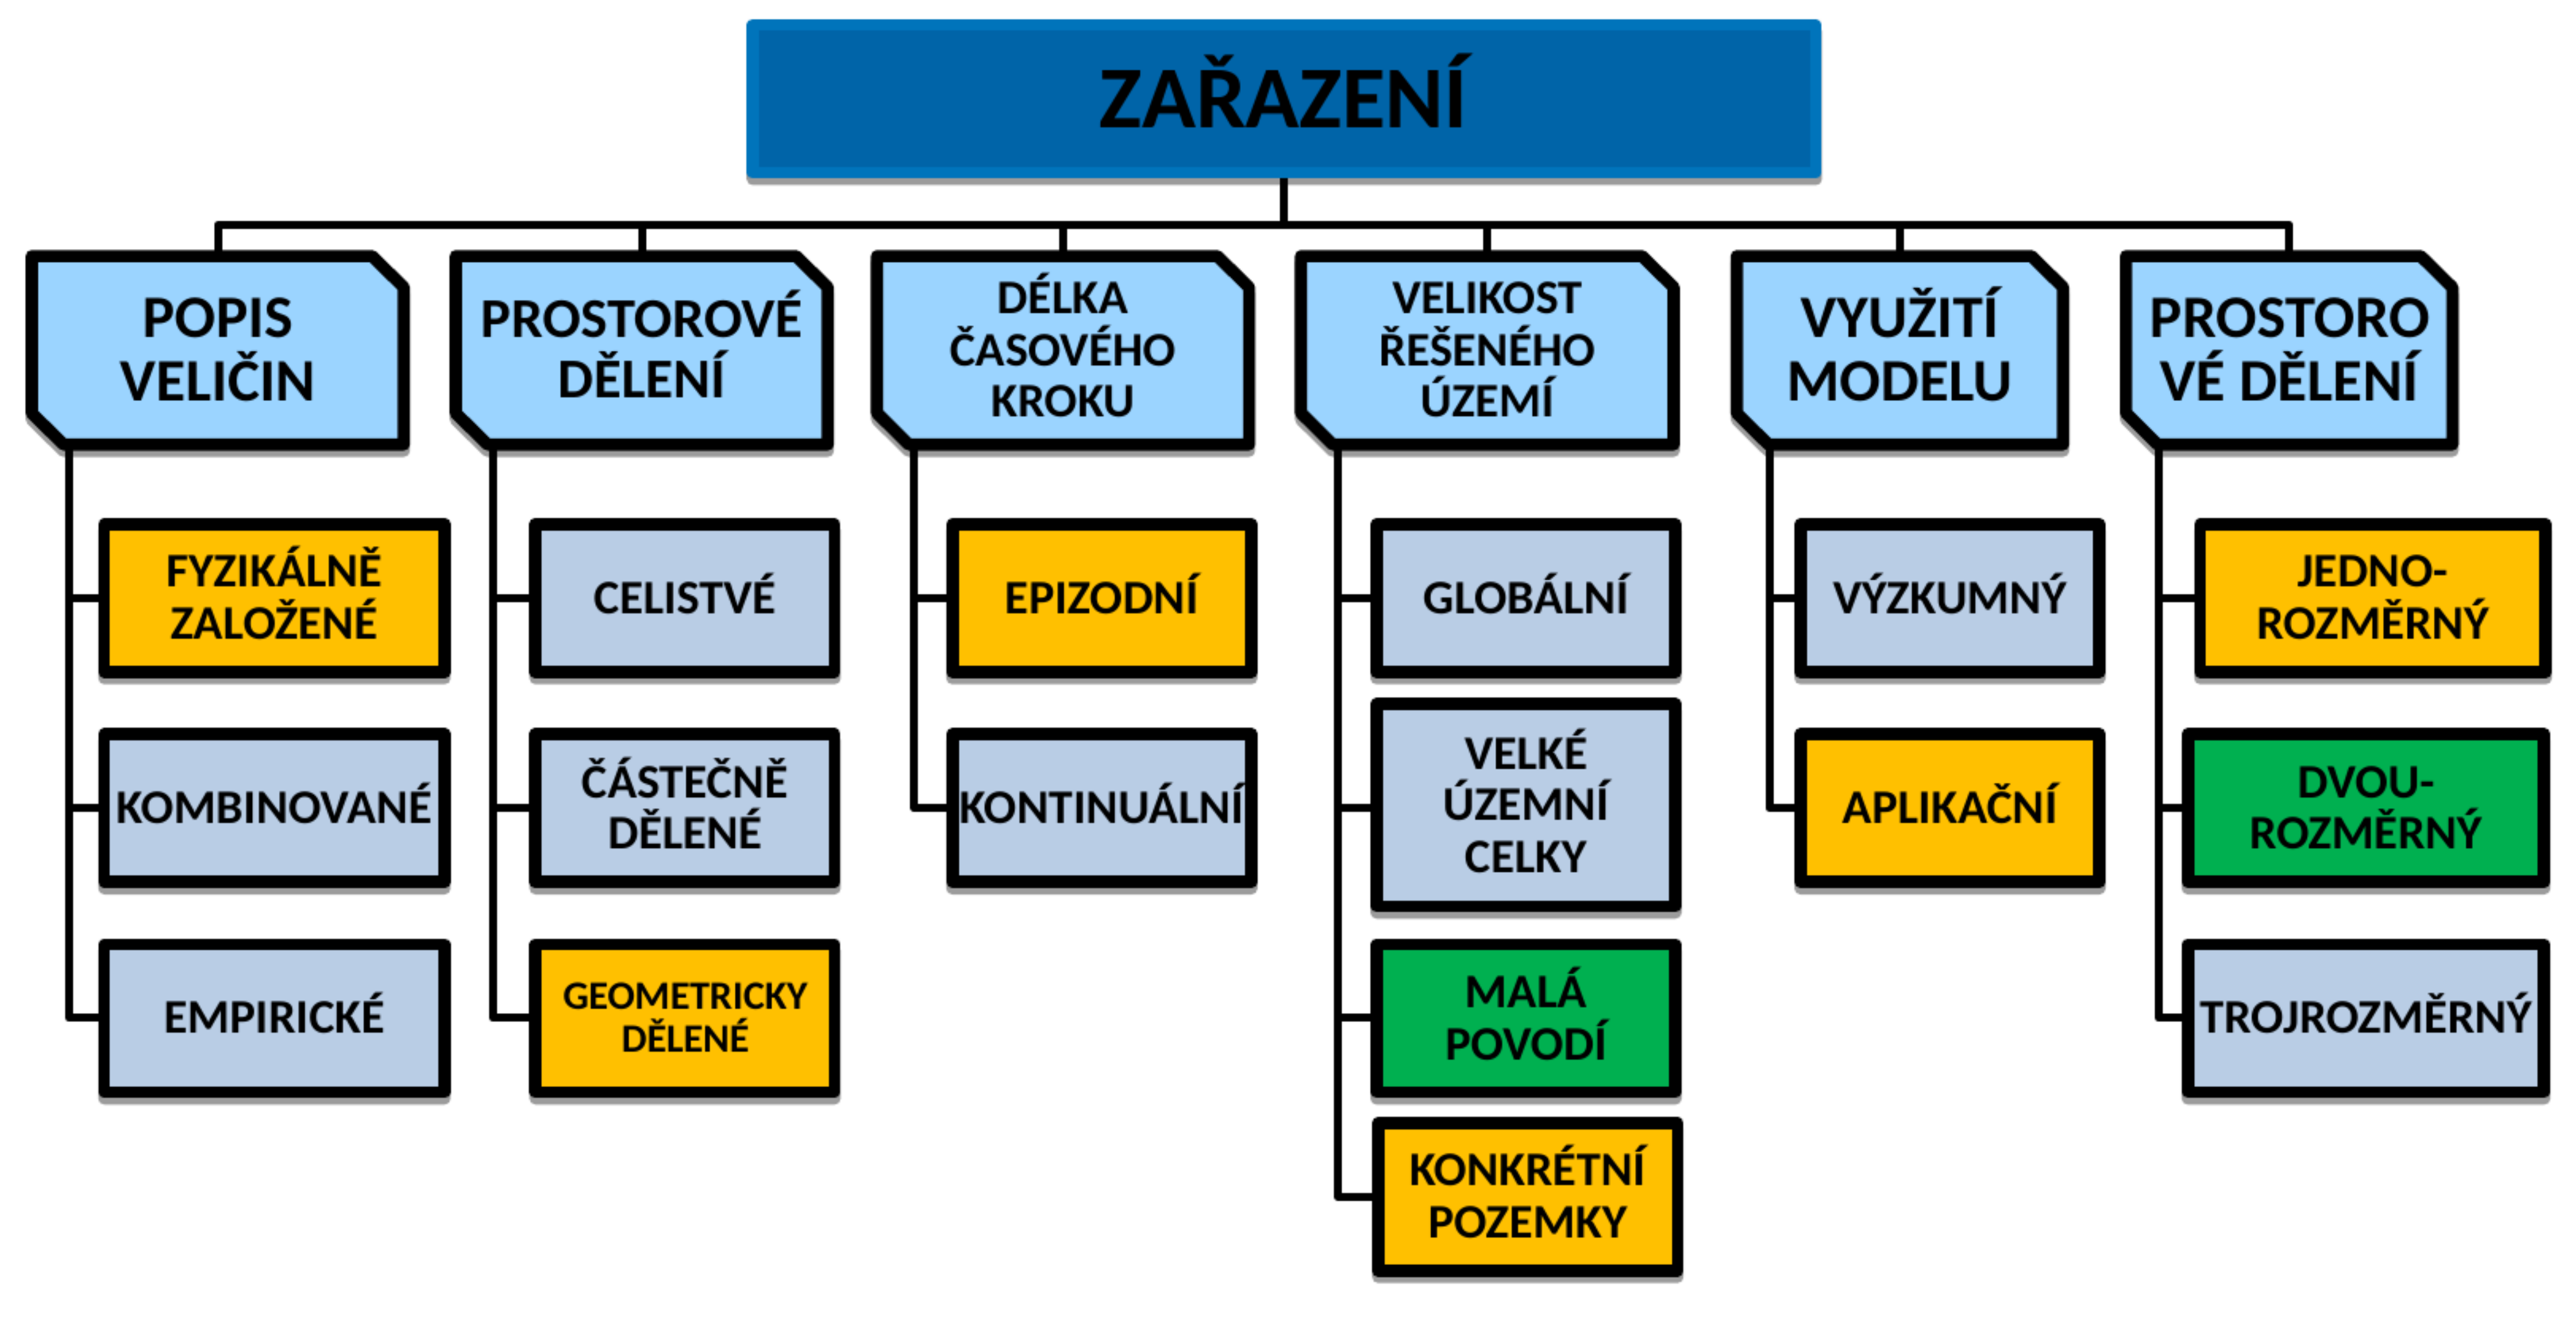
\includegraphics[width=\textwidth]{obr/vyuziti.png}
    \end{frame}

    \begin{frame}{SMODERP}
        Součást několika předpisů\\[1em]
        \begin{itemize}
            \item DOS T 3.17 - Protierozní ochrana, Váška, J., Informační centrum ČKAIT, Praha, 2000
            \item ČSN 75 4500 -  Protierozní ochrana zemědělské půdy, Český normalizační institut, 1996
            \item Janeček M., Ochrana zemědělské půdy před erozí - metodika, např. 2007, 2012
            \item Metodiky TPEO, Kadlec (2014), Dostál (2014)
            \item Kavka P., - Krátkodobé srážky pro hydrologické modelování a navrhování drobných vodohospodářských staveb v krajině, 2018
        \end{itemize}
    \end{frame}

